\chapter{Background Theory}
\section{Reference Frames}
The main reference frames that are relevant for navigation and control are ECEF, NED and BODY. A brief introduction to these reference frames based on \citep{Fossen} and \citep{vik} follows. Denavit-Hartenberg convention (DH convention) is a useful tool for defining reference frames. A brief introduction to DH convention based on \citep{Spong} follows.
\subsubsection{ECEF}
The Earth-centered Earth-fixed (ECEF) reference frame has its origin fixed to the center of the earth while rotating with the earth. The x-axis is defined to point at the intersection between the $0^{\circ}$ longitude and the $0^{\circ}$ latitude. The z-axis points along the earths rotation axis and the y-axis complete the right handed orthogonal coordinate system.\\\newline
The position in the ECEF frame can be expressed both with Cartesian coordinates ($x_e$, $y_e$, $z_e$) and with ellipsoidal coordinates (longitude ($l$), latitude ($\mu$), height ($h$)). The transformation from Cartesian ECEF-coordinates to ellipsoidal ECEF-coordinates is given by
\begin{eqnarray}
\begin{bmatrix}
x_e\\
y_e\\
z_e
\end{bmatrix}  = \begin{bmatrix}
(N + h)\cos \mu \cos l\\
(N + h)\cos \mu \sin l\\
(\dfrac{r_p^2}{r_e^2}N + h) \sin \mu
\end{bmatrix}
\end{eqnarray}
where $r_e$ = 6378137 m is the equatorial radius of ellipsoid and $r_p$ = 6356752 m is the polar axis radius of the ellipsoid as defined in WGS-84. The parameter $N$ is the radius of curvature in prime vectorial obtained from \citep{vik}. 
\begin{eqnarray}
N = \dfrac{r_e^2}{\sqrt{r_e^2 \cos ^2 \mu + r_p^2 \sin ^2 \mu}}
\end{eqnarray}
The transformation from Cartesian coordinates to ellipsoid coordinates is a bit more complicated. Longitude is calculated straight forward as
\begin{eqnarray}
l = \tan ^{-1} (\dfrac{y_e}{x_e})
\end{eqnarray}
but the calculations of latitude  and height are implicit equations
\begin{eqnarray}
\tan(\mu) &=& \dfrac{z}{p}(1 - e^2\dfrac{N}{N + h})^{-1}\\
h &=& \dfrac{p}{\cos(\mu)} - N
\end{eqnarray}
where $e$ is the eccentricity of the Earth given by
\begin{eqnarray}
e = \sqrt{1 - (\dfrac{r_p}{r_e})^2}
\end{eqnarray}
There are several algorithms that can be used to solve these implicit equations, see for instance Algorithm 2.4 in \citep{Fossen}.
\subsubsection{NED}
The north-east-down (NED) reference frame is moving with the body. The x-axis is always pointing north, the y-axis is pointing east and the z-axis i pointing down normal to the Earth surface.
\subsubsection{BODY}
The BODY reference frame is body fixed and rotates and moves with the body. It is usually defined with the x-axis pointing along the longitudinal axis, the y-axis pointing along the transversal axis and the z-axis pointing along the normal axis of the body.
\subsubsection{Transformation Between ECEF and NED}
A vector defined in NED can be transformed to the ECEF frame by the use of a rotation matrix that defines the relationship between NED and ECEF reference frames.
\begin{eqnarray}
\boldsymbol{p}^e = \boldsymbol{R}_n^e(\boldsymbol{\Theta} _{en})\boldsymbol{p}^n\\
\boldsymbol{\Theta} _{en} = \begin{bmatrix}
l & \mu & h\\
\end{bmatrix}^T
\label{ecef}
\end{eqnarray}
Where $\boldsymbol{R}_n^e(\boldsymbol{\Theta} _{en})$ is found by first performing a rotation $l$ about the z-axis and then a rotation $(-\mu -\dfrac{\pi}{2})$ about the y-axis. This gives
\begin{eqnarray}
\boldsymbol{R} _n^e(\boldsymbol{\Theta} _{en}) = \begin{bmatrix}
-\cos(l)\sin(\mu) & -\sin(-l) & -\cos(l)\cos(\mu)\\
-\sin(l)\sin(\mu) & \cos(l) & -\sin(l)\cos(\mu)\\
\cos(\mu) & 0  & -\sin(\mu)\\
\end{bmatrix} 
\end{eqnarray}
\subsubsection{Transformation Between NED and BODY}
A vector defined in BODY can be transformed to the NED frame by the use of the Euler angle rotation matrix.
\begin{eqnarray}
\boldsymbol{p}^n = \boldsymbol{R}_b^n(\boldsymbol{\Theta}_{nb})\boldsymbol{p}^b
\end{eqnarray}
Where $\boldsymbol{\Theta}_{nb} = \begin{bmatrix}
\phi & \theta & \psi\\
\end{bmatrix}^T$ are the Euler angles roll, pitch and yaw. 
\begin{eqnarray}
\boldsymbol{R} _b^n(\boldsymbol{\Theta}_{nb}) = 
\begin{bmatrix}
c_\psi c_\theta & -s_\psi c_\phi + c_\psi s_\theta s_\phi & s_\psi s_\phi + c_\psi c_\phi s_\theta\\
s_\psi c_\theta & c_\psi c_\phi + s_\phi s_\theta s_\psi & -c_\psi s_\phi + s_\theta s_\psi c_\phi\\
-s_\theta & c_\theta s_\phi & c_\theta c_\phi
\end{bmatrix}
\label{R_ned}
\end{eqnarray}
The notation s and c with an angle as subscript is used to represent $\sin (angle)$ and $cos (angle)$ respectively. This notation is used throughout this report.
\subsubsection{Denavit-Hartenberg Convention}
The DH convention is a systematic procedure for relating orientation and position of different reference frames, and a tool to select frames. The homogeneous transformation $A_i$ (the transformation matrix from reference system $i-1$ to reference system $i$) is represented as a product of four basic transformations 
\begin{eqnarray}
\boldsymbol{A}_i &=& \boldsymbol{Rot}_{z,\theta _i}\boldsymbol{Trans}_{z, d_i}\boldsymbol{Trans}_{x, a_i}\boldsymbol{Rot}_{x, \alpha -i}\nonumber\\
 &=& \begin{bmatrix}
c_{\theta _i} & -s_{\theta _i} & 0 & 0\\
s_{\theta _i} & c_{\theta _i} & 0 & 0\\
0 & 0 & 1 & 0\\
0 & 0 & 0 & 1
\end{bmatrix}
\begin{bmatrix}
1 & 0 & 0 & 0\\
0 & 1 & 0 & 0\\
0 & 0 & 1 & d_i\\
0 & 0 & 0 & 1
\end{bmatrix}
\begin{bmatrix}
1 & 0 & 0 & a_i\\
0 & 1 & 0 & 0\\
0 & 0 & 1 & 0\\
0 & 0 & 0 & 1
\end{bmatrix}
\begin{bmatrix}
1 & 0 & 0 & 0\\
0 & c_{\alpha _i} & -s_{\alpha _i} & 0\\
0 & s_{\alpha _i} & c_{\alpha _i} & 0\\
0 & 0 & 0 & 1
\end{bmatrix}\nonumber\\
&=& \begin{bmatrix}
c_{\theta _i} & -s_{\theta _i} c_{\alpha _i} & s_{\theta _i} s_{\alpha _i} & a_ic_{\theta _i}\\
s_{\theta _i} & c_{\theta _i} c_{\alpha _i} & -c_{\theta _i} s_{\alpha _i} & a_is_{\theta _i}\\
0 & s_{\alpha _i} & c_{\alpha _i} & d_i\\
0 & 0 & 0 & 1
\end{bmatrix}
\label{DH}
\end{eqnarray}
where $\theta_i$ is rotation around the z-axis, $d_i$ is transversal movement along the z-axis, $a_i$ is the transversal movement along the new x-axis direction and $\alpha_i$ is the rotation around the new x-axis direction. There exists unique values of $\theta_i$, $d_i$, $a_i$ and $\alpha_i$ to make equation (\ref{DH}) valid if the frames have the features:
\begin{itemize}
\item The axis $x_i$ is perpendicular to the axes $z_{i-1}$
\item The axis $x_i$ intersects the axis $z_{i-1}$
\end{itemize}
The transformation matrix $T_j^i$ expresses the position and orientation of frame $o_jx_jy_jz_j$ with respect to frame $o_ix_iy_iz_i$ and is calculated as
\begin{equation}
  \boldsymbol{T}_j^i=\begin{cases}
    \boldsymbol{A}_{i+1}\boldsymbol{A}_{i+2}...\boldsymbol{A}_{j-1}\boldsymbol{A}_j & \text{if $i<j$}\\
    I & \text{if $i=j$}\\
    (\boldsymbol{T}_i^j)^{-1} & \text{if $j>i$}
  \end{cases}
\end{equation}
$\boldsymbol{T}_j^i$ for $i<j$ contain a rotation matrix $\boldsymbol{R}_i^j$ from frame $i$ to $j$ and the position $\boldsymbol{o}_j^i$ of the origin of frame j with respect to frame i.
\begin{eqnarray}
\boldsymbol{T}_j^i = \begin{bmatrix}
\boldsymbol{R}_j^i & \boldsymbol{o}_j^i\\
0 & 1
\end{bmatrix}
\label{T}
\end{eqnarray}  
\section{Computer Vision}
\subsection{OpenCV}\label{opencv}
OpenCV (Open Source Computer Vision Library) is an open source computer vision and machine learning software library that has more than 2500 optimized algorithms \citep{opencv}. A few of these algorithms will be briefly explained here. The ones explained are the most relevant for object recognition.
\subsubsection{Color Recognition}
A digital picture is essentially a matrix of values describing the picture. This matrix is dependent of the color space the picture is defined in. A picture captured from for instance a web-camera is defined in the BGR (Blue-Green-Red) color space, which means that the colors in the picture are defined by combinations of these colors. The color is defined by the relationship between these values, while the brightness is defined by how high these values are. Hence it could be difficult to select threshold values if one is looking for an object of a specific color, because different light conditions would give very different values for the color. To make the thresholding more intuitive one can transform the picture into the HSV (Hue-Saturation-Value) color space. The hue value is unique for a specific color and describes the base color. The saturation describes the strength of the color and the value is a measure of brightness. This makes it simpler to find intuitive thresholds for specific object colors that can handle different lightning conditions. An visualization of the HSV-color space is found in Figure \ref{hsvWheel}. 
\begin{figure}[H]
\centering
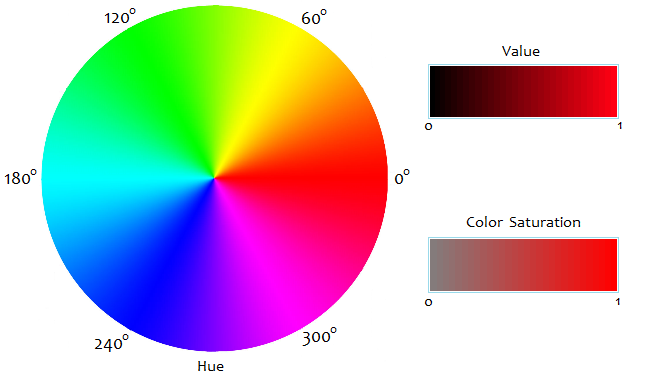
\includegraphics[width = 8cm]{fig/hsv.png}
\caption{HSV-color wheel \textit{Courtesy of had2know.com}}
\label{hsvWheel}
\end{figure}\noindent
The HSV-picture is thresholded with the desired intervals of the HSV-values. This results in a binary image where the pixel values are one if the color is found and zero if the color is different than the desired color. With good choices of colors for the object and the thresholding values, one would get a good understanding of where the object is.
\subsubsection{Canny Edge Detector and Moments}
The Canny Edge Detector uses an algorithm presented in \citep{canny} that detects edges. It can be used to detect contours. If the Canny Edge Detector is used on a binary image like the one described in the previous section it would find the contour surrounding the area of the detected object.\\\newline
Then this contour could be fed to the moment function in OpenCV which calculates the center of moment for the contour, which is the center of the outline of the object.
\subsubsection{Cascade Classifier}
The use of cascade classifiers includes two major stages, training and detection \citep{cascade}. Training is executed once only, while detection is executed run time. Training takes two different sets of samples, positive and negative samples. The positive samples are samples containing the object, while the negative samples are samples without the object. These samples are run through a cascade classifier to create a ``rule" of what to look for in the detection phase.\\\newline
There exists several different cascade classifiers, two of these are implemented in OpenCV. These are Haar- and LBP-classifiers. They use different features and have different runtime. Details on these algorithm are outside the scope of this text.\\
\newline
Accuracy of the use of cascade classifiers is dependent on the object to be detected, and the number of samples used for training. For instance one positive sample can be sufficient for detection of a rigid object, while detection of for instance faces will need hundreds or even thousands of positive samples.\\\newline
There are tools in OpenCV that take the positive samples and creates many new positive samples of it. This is done by randomly rotating the object around all three axes, changing the objects intensity and placing it on random backgrounds \citep{cascade}.
\subsubsection{SURF}
Speeded Up Robust Features (SURF) is a further development and speeded up algorithm on the basis of SIFT (Scale-Invariant Feature Transform) \citep{surf}. These algorithms use a single picture of the object for the recognition. Based on different techniques beyond the scope of this text, key points are found describing the object. The key points is assigned an orientation to achieve invariance to image rotation, and the way the key point is selected make the algorithm scale invariant \citep{sift}.\\\newline
For commercial use one should note that both SURF and SIFT is patented and part of a non-free module in OpenCV.